%! suppress = MissingImport
In this section, you will install the ``slider'' switches that toggle between their two positions, holding their position until toggled again.
We will wire them such that when a switch is toggled to the left, it will produce a 0, and when it is toggled to the right, it will produce a 1.
Figure~\ref{fig:switch-diagram} shows a diagram of the wiring for the slider switches.

%! suppress = NonMatchingIf
\begin{figure}[p]
    \centering
    \ifdefstring{\serialprotocol}{SPI}{
        \subfloat[3-pin switches]{
            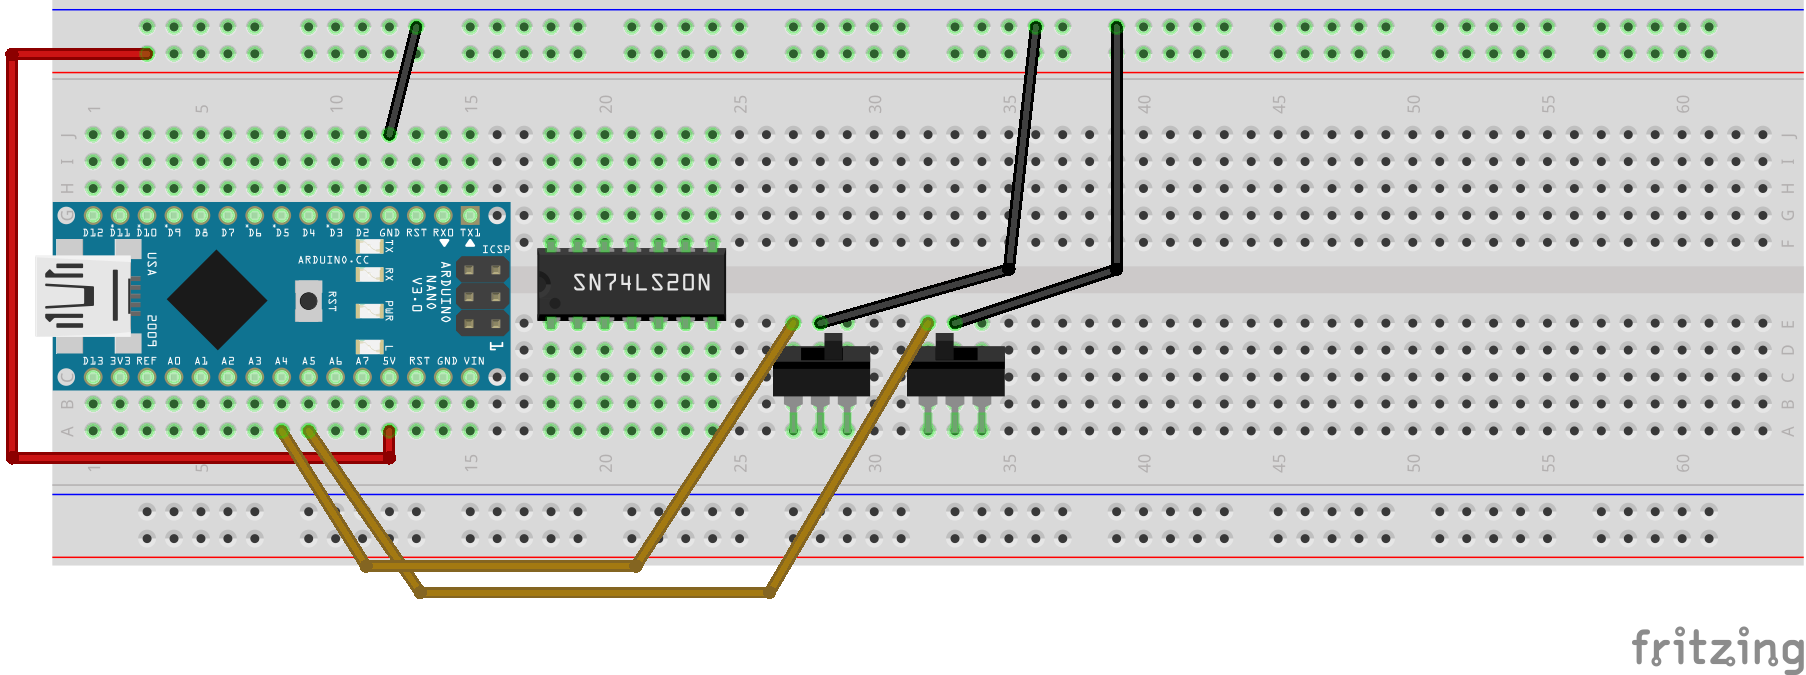
\includegraphics[width=0.9\textwidth]{fritzing_diagrams/switch-spi-spdt}
        }
%        \hfil
%        \subfloat[2-pin switches]{
%            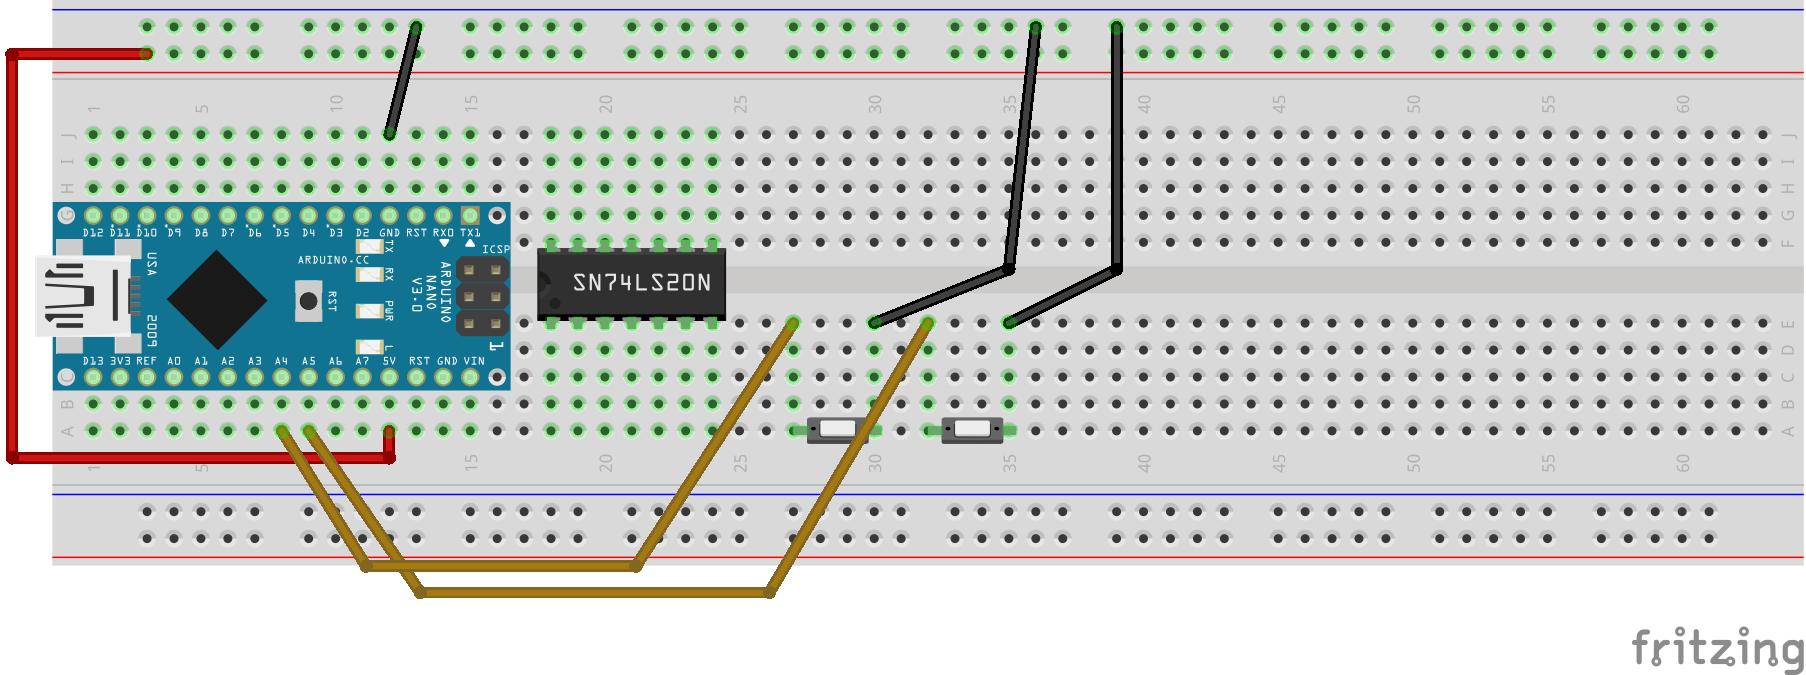
\includegraphics[width=0.9\textwidth]{fritzing_diagrams/switch-spi-dip1}
%        }
    }{}
    \ifdefstring{\serialprotocol}{I2C}{
        \subfloat[3-pin switches]{
            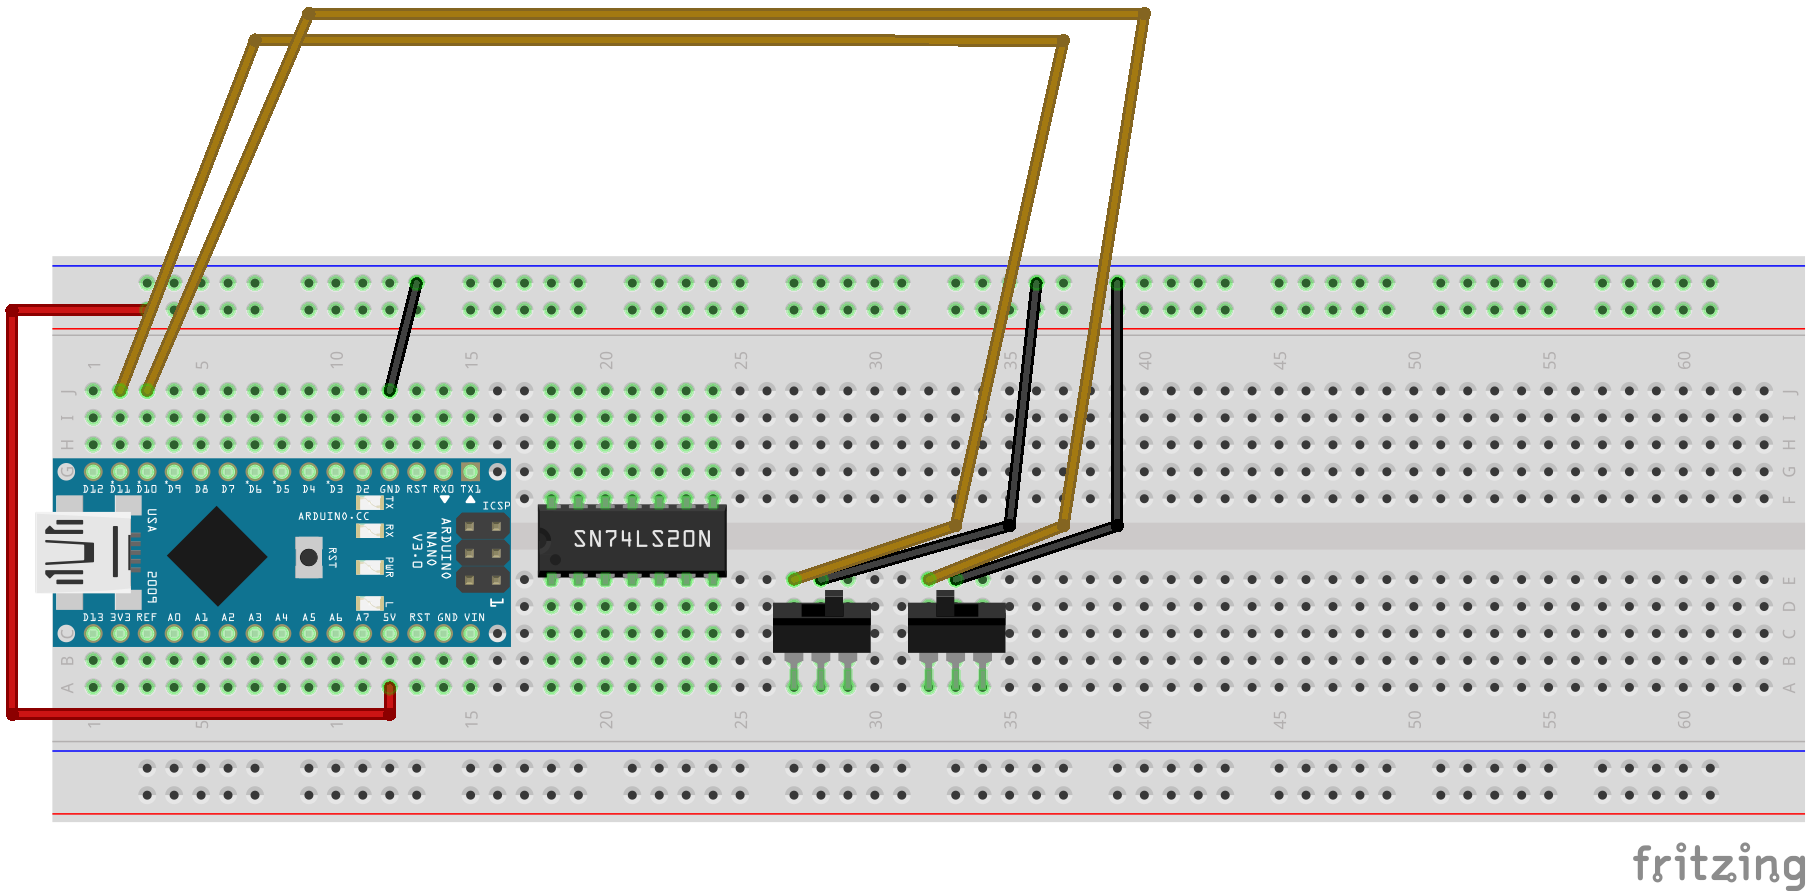
\includegraphics[width=0.9\textwidth]{fritzing_diagrams/switch-i2c-spdt}
        }
%        \hfil
%        \subfloat[2-pin switches]{
%            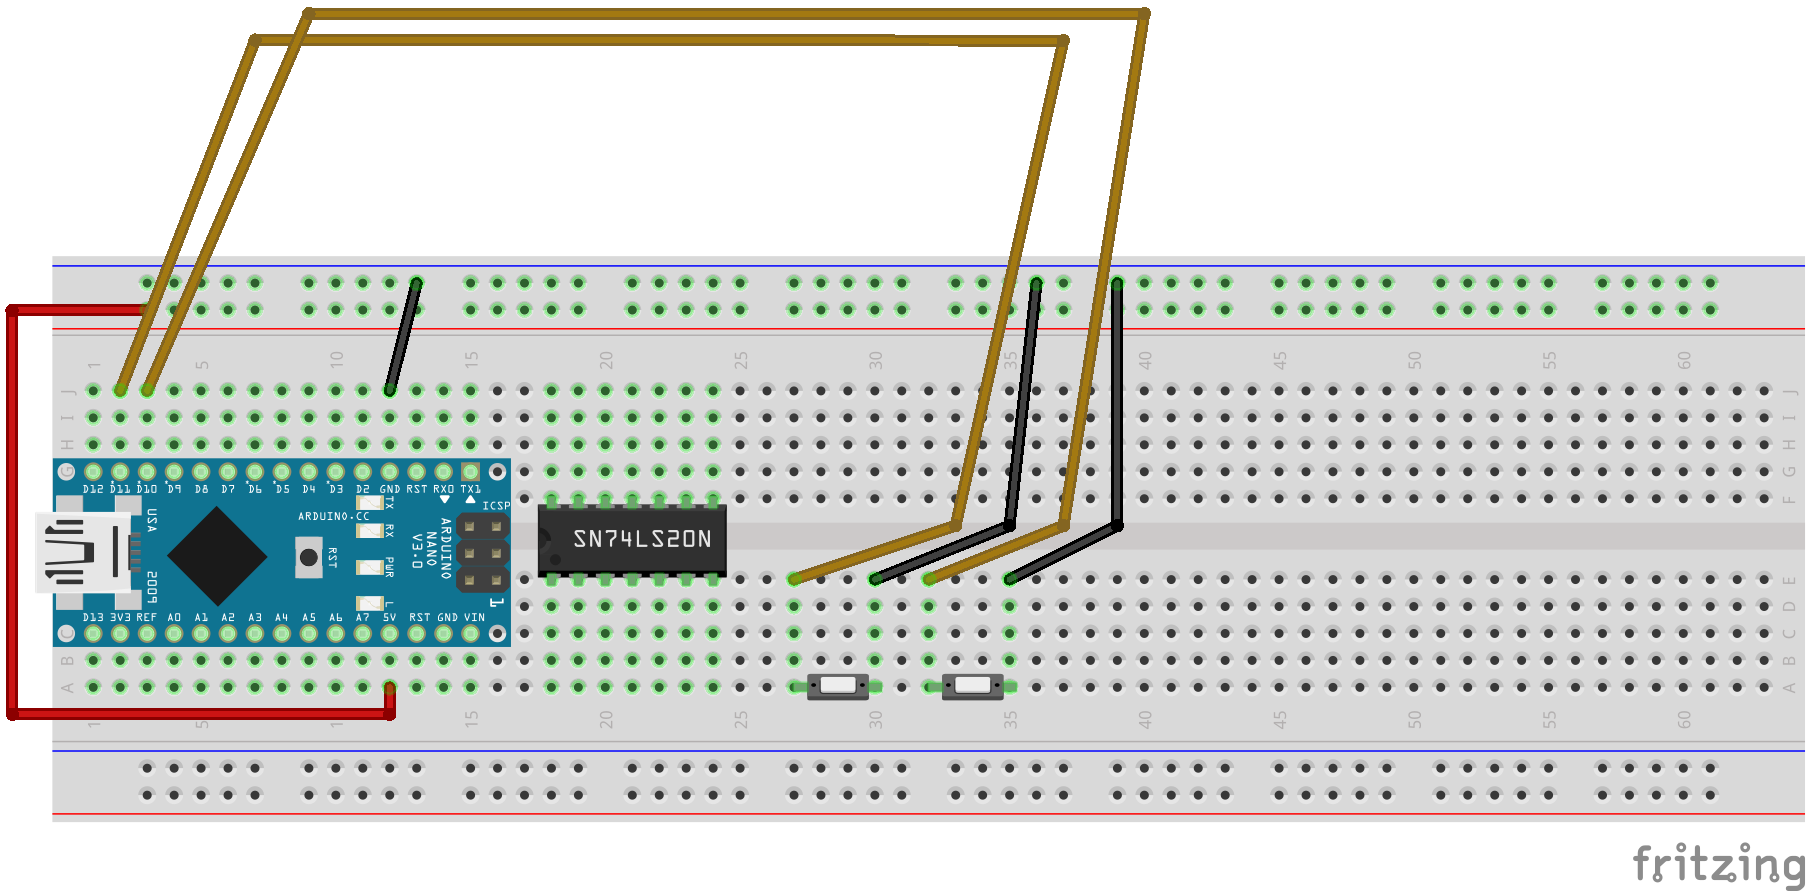
\includegraphics[width=0.9\textwidth]{fritzing_diagrams/switch-i2c-dip1}
%        }
    }{}
    \caption{Diagram of wiring associated with toggle switch input.
        \label{fig:switch-diagram}}
\end{figure}

\disconnect\

%\prepunch{a\controlrow{1} and a\controlrow{6}}
%If you have 3-pin switches, then pre-punch holes into contact points a\controlrow{2}, a\controlrow{3}, a\controlrow{7} and a\controlrow{8}.
%If you have 2-pin switches, then pre-punch holes into contact points a\controlrow{4} and a\controlrow{9}.
\begin{description}
    \checkoffitem{\prepunch{a\controlrow{1}--a\controlrow{3} and a\controlrow{6}--a\controlrow{8}}}

    \checkoffitem{Insert one slider switch into contact points a\controlrow{1}--a\controlrow{3}.} % (for 3-pin switches) or contact points a\controlrow{1}--a\controlrow{4} (for 2-pin switches).
    \checkoffitem{Place the other slider switch into contact points a\controlrow{6}--a\controlrow{8}.} % (for 3-pin switches) or contact points a\controlrow{6}--a\controlrow{9} (for 2-pin switches).
\end{description}
For the two wires that will connect the switches to the \developmentboard, you can use 10cm jumpers (especially if that is all that you have);
however, if you use 20cm jumpers, then in Section~\ref{sec:keypad} we will show how to keep some wires away from the controls.
\begin{description}
    \checkoffitem{Peel off one wire from the \rainbow\ and use it to connect contact point e\controlrow{1} (electrically connected to the left switch's left pin) to contact point \mculeftswitchpoint\ (electrically connected to the \developmentboard's \mculeftswitch\ pin).}
    \checkoffitem{Peel off another wire from the \rainbow\ and use it to connect contact point e\controlrow{6} (electrically connected to the right switch's left pin) to contact point \mcurightswitchpoint\ (electrically connected to the \developmentboard's \mcurightswitch\ pin).}

    \checkoffitem{Peel off two more wires from the \rainbow.}
\end{description}
You will use these to connect the switches center pins %(for 3-pin switches) or right pins (for 2-pin switches)
to the upper \ground.
Specifically,
\begin{description}
    \checkoffitem{Place the end of one wire into contact point e\controlrow{2}.} %(for 3-pin switches) or e\controlrow{4} (for 2-pin switches);
    \checkoffitem{Place the other end of that wire into the upper \ground.}
    \checkoffitem{Now place the end of the other wire into contact point e\controlrow{7}.} %(for 3-pin switches) or e\controlrow{9} (for 2-pin switches);
    \checkoffitem{Place the other end of that wire into the upper \ground.}
\end{description}
The switches' right pins will not be electrically connected to anything.

%If you have 3-pin switches, the switches' right pins will not be electrically connected to anything.

%TODO: parameterize for I2C vs SPI; add spdt vs dip1 close-ups
\begin{figure}
    \centering
    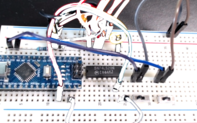
\includegraphics[width=0.6\textwidth]{direct/switches/switch-spdt-i2c}
    \caption{The slider switches, each with one pin grounded, one pin connected to the \developmentboard, and one pin floating.
        \label{fig:switch-spdt}}
\end{figure}

When you have finished setting up the switches' wiring, there should be the
electrical connections described in Table~\ref{tab:switch-spdt}.% or \ref{tab:switch-dip1}.

\begin{table}
    \begin{center}\begin{tabular}{||c|c|c||} \hline\hline
    Switch                      & \developmentboard\ pin    & Pulled High/Low \\ \hline
    Left switch's left pin      & \mculeftswitch    & \\
    Left switch's center pin    &                   & \ground\ \\
    Left switch's right pin     & \multicolumn{2}{c||}{not connected / floating} \\
    Right switch's left pin     & \mcurightswitch   & \\
    Right switch's center pin   &                   & \ground \\
    Right switch's right pin    & \multicolumn{2}{c||}{not connected / floating} \\ \hline\hline
    \end{tabular}\end{center}
    \caption{Electrical Connections for 3-pin Slider Switches.
        \label{tab:switch-spdt}}
\end{table}

%\begin{table}
%    \begin{center}\begin{tabular}{||c|c|c||} \hline\hline
%    Switch                      & \developmentboard\ pin    & Pulled High/Low \\ \hline
%    Left switch's left pin      & \mculeftswitch    & \\
%    Left switch's right pin     &                   & Pulled Low \\
%    Right switch's left pin     & \mcurightswitch   & \\
%    Right switch's right pin    &                   & Pulled Low \\ \hline\hline
%    \end{tabular}\end{center}
%    \caption{Electrical Connections for 2-pin Slider Switches.
%        \label{tab:switch-dip1}}
%\end{table}

\checkpoint{inserted and wired the slider switches}

Connect your \developmentboard\ to the computer.
In the IDE's Serial Monitor, notice that Left~switch is LEFT when the left switch is toggled to the left, and it is RIGHT when the left switch is toggled to the right.
Similarly, Right~switch is LEFT or RIGHT, depending on whether the right switch is toggled to the left or right.